\documentclass{article}
\usepackage{fullpage}
\usepackage{graphicx}

\title{Grid Unit Four-way 2000x1200 0.35}
\date{\today}

\begin{document}
\maketitle

\begin{figure}
\begin{center}
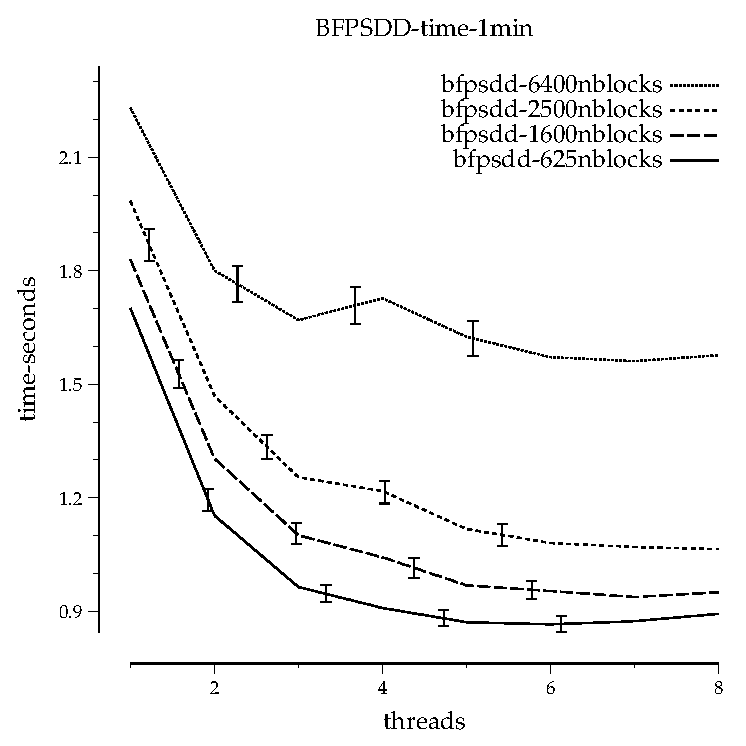
\includegraphics{BFPSDD-time-1min}
\end{center}
\caption{BFPSDD}
\end{figure}

\begin{figure}
\begin{center}
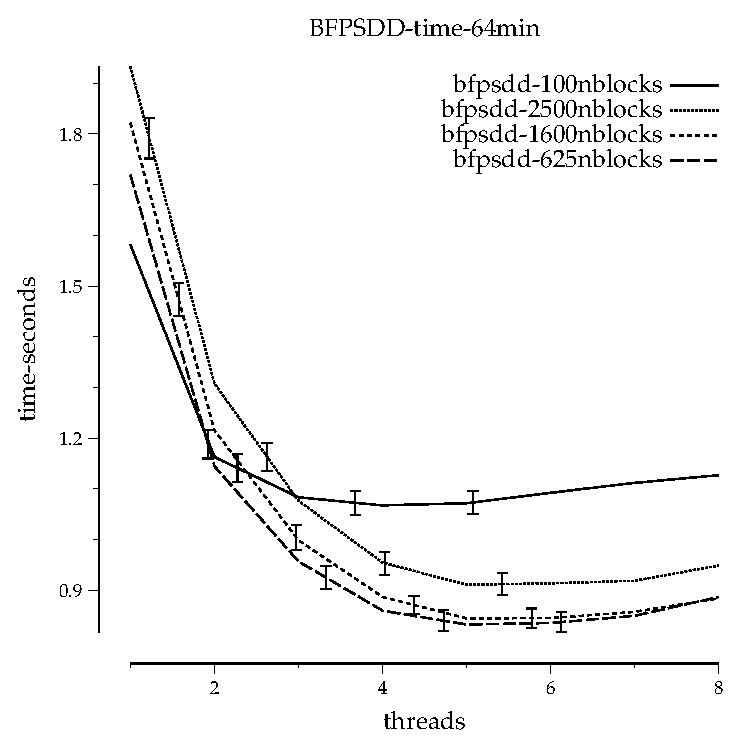
\includegraphics{BFPSDD-time-64min}
\end{center}
\caption{BFPSDD 64 minimum expansions}
\end{figure}

\begin{figure}
\begin{center}
\includegraphics[width=2in]{BFPSDD-delta-time-delta=256}
\includegraphics[width=2in]{BFPSDD-delta-time-delta=512}
\includegraphics[width=2in]{BFPSDD-delta-time-delta=1024}
\includegraphics[width=2in]{BFPSDD-delta-time}
\end{center}
\caption{BFPSDD using the delta-f modification}
\end{figure}

\begin{figure}
\begin{center}
\includegraphics{BFPSDD-nthreads-time}
\end{center}
\caption{BFPSDD using the 4*nthreads minimum free nblocks modification}
\end{figure}

%%% DYNPSDD

\begin{figure}
\begin{center}
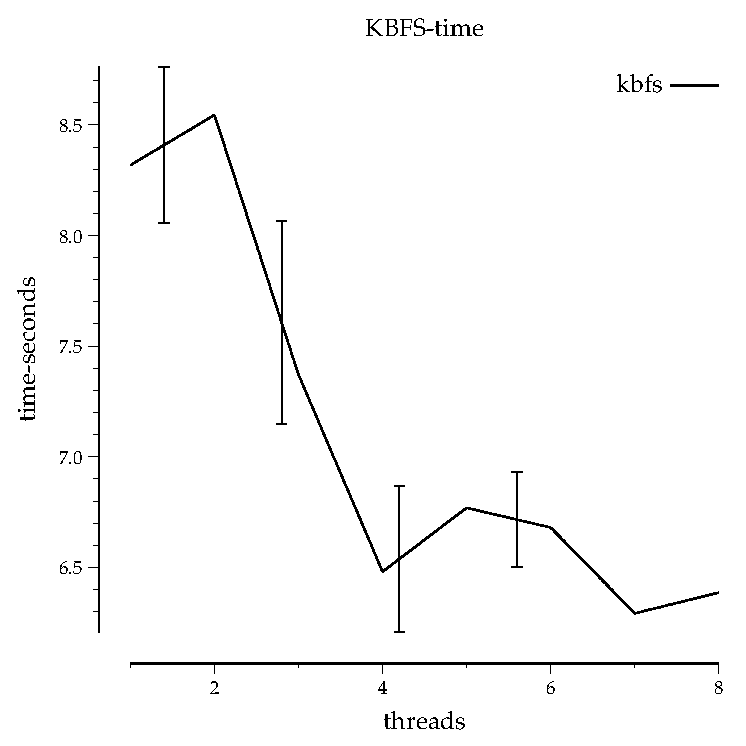
\includegraphics{KBFS-time}
\end{center}
\caption{KBFS}
\end{figure}

\begin{figure}
\begin{center}
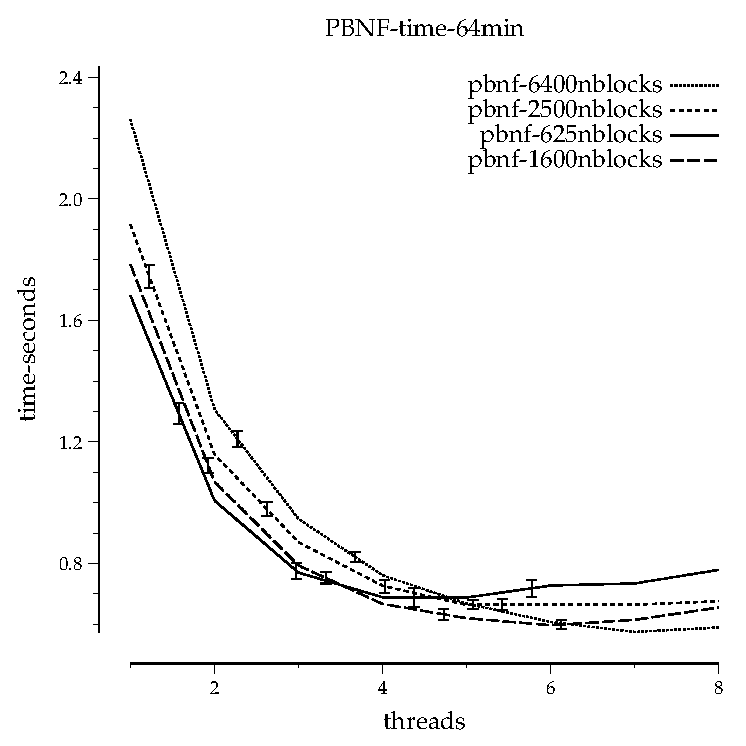
\includegraphics{PBNF-time-64min}
\end{center}
\caption{PBNF}
\end{figure}

\begin{figure}
\begin{center}
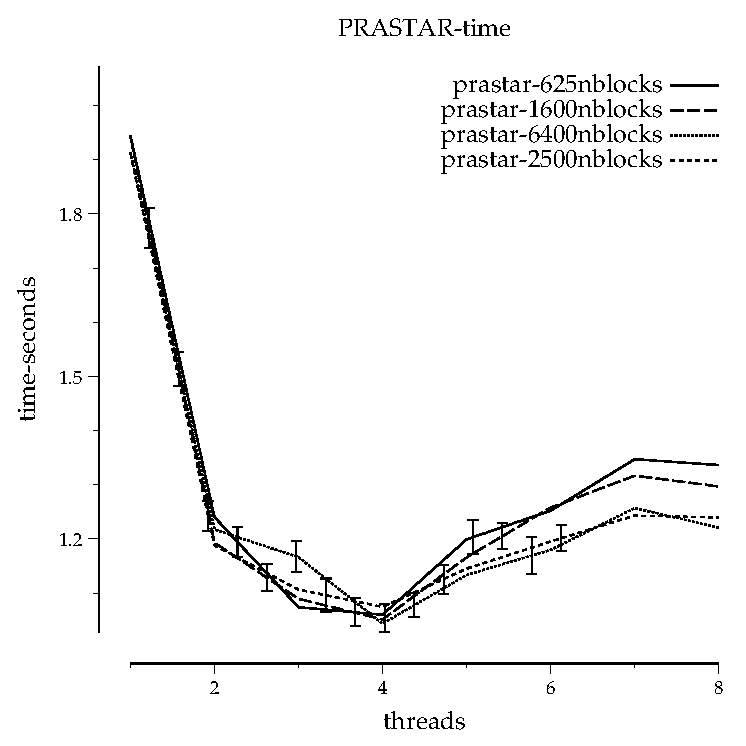
\includegraphics{PRASTAR-time}
\end{center}
\caption{PRASTAR}
\end{figure}

\begin{figure}
\begin{center}
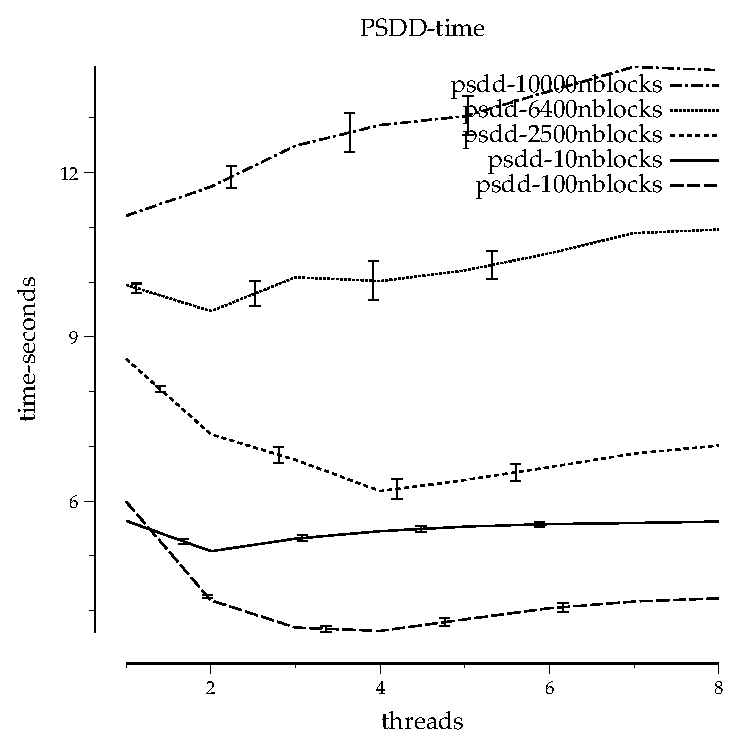
\includegraphics{PSDD-time}
\end{center}
\caption{PSDD}
\end{figure}

\begin{figure}
\begin{center}
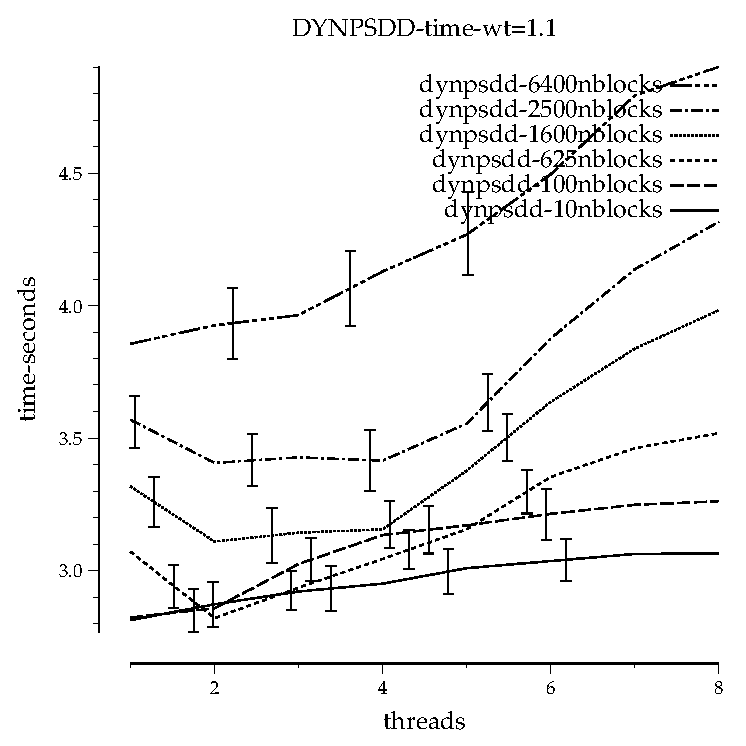
\includegraphics[width=2.5in]{DYNPSDD-time-wt=1.1.eps}
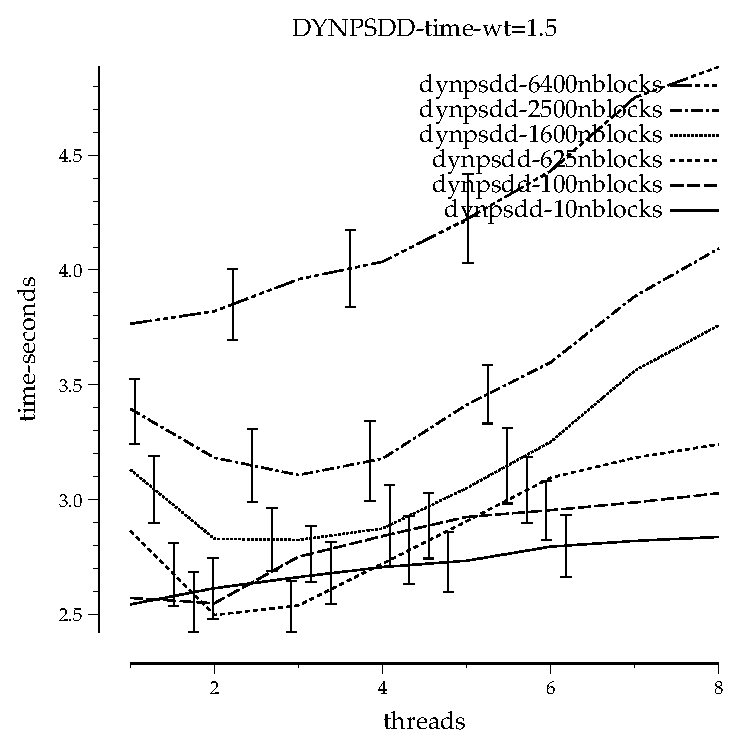
\includegraphics[width=2.5in]{DYNPSDD-time-wt=1.5.eps}
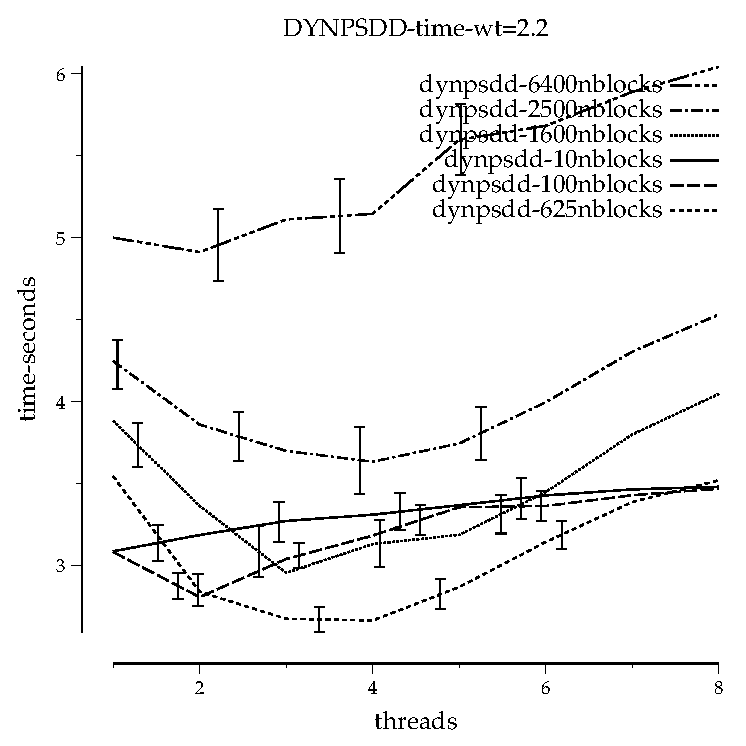
\includegraphics[width=2.5in]{DYNPSDD-time-wt=2.2.eps}
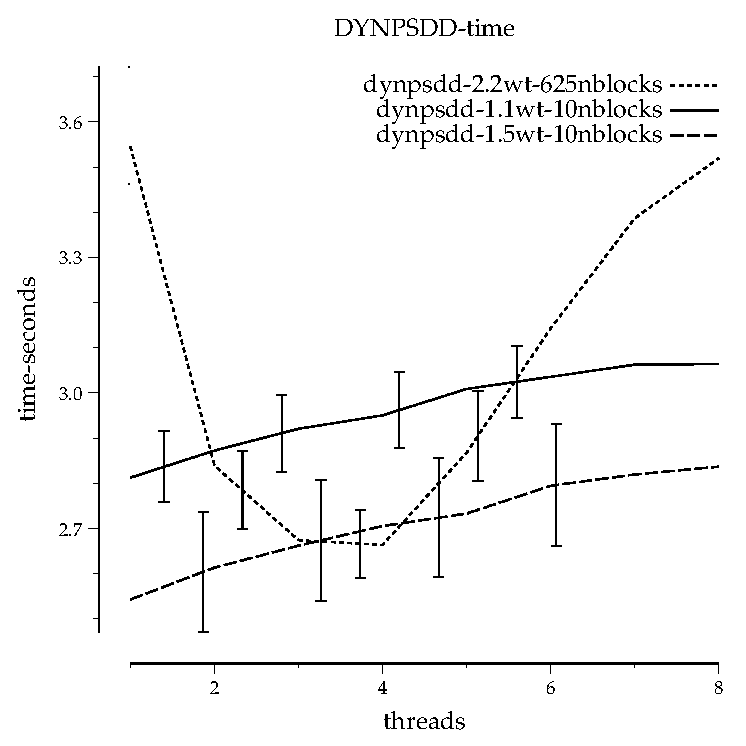
\includegraphics[width=2.5in]{DYNPSDD-time}
\end{center}
\caption{DYNPSDD}
\end{figure}

\begin{figure}
\begin{center}
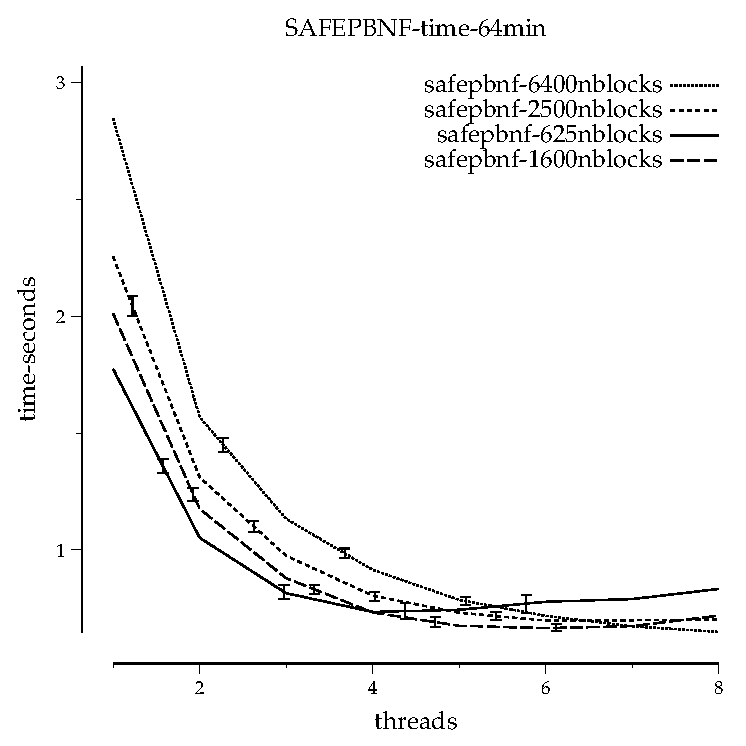
\includegraphics{SAFEPBNF-time-64min}
\end{center}
\caption{SAFEPBNF}
\end{figure}

\begin{figure}
\begin{center}
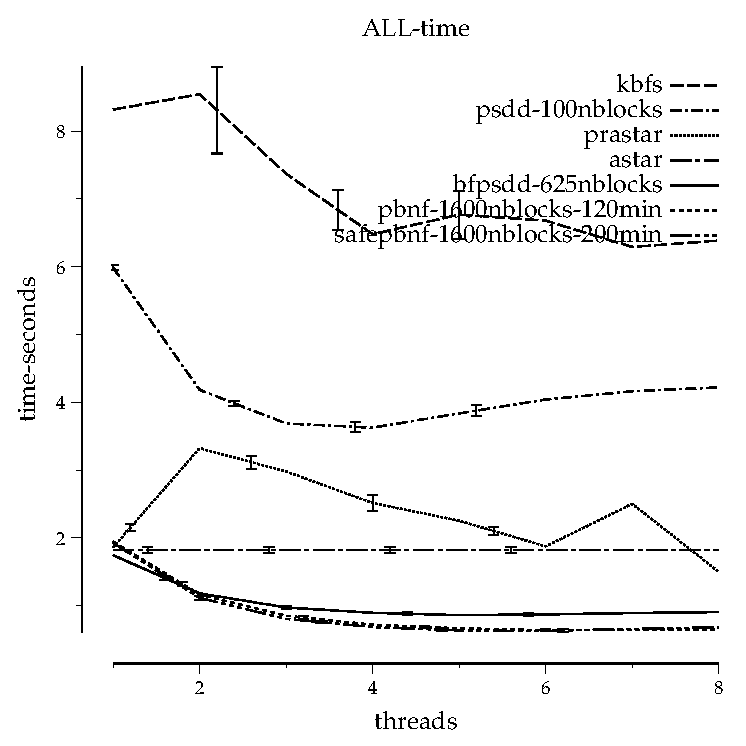
\includegraphics{ALL-time}
\end{center}
\caption{All algorithms}
\end{figure}

\begin{figure}
\begin{center}
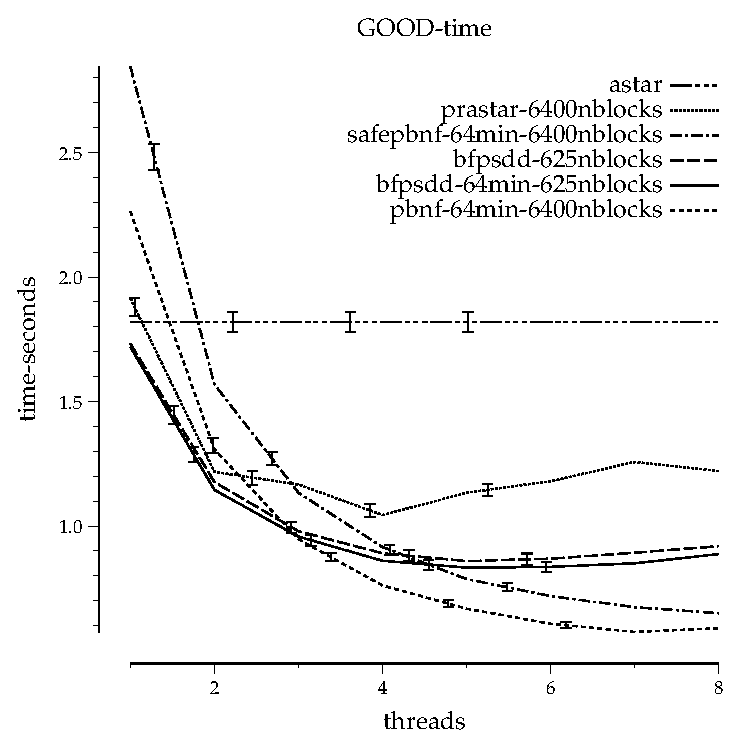
\includegraphics{GOOD-time}
\end{center}
\caption{The best few algorithms}
\end{figure}

\end{document}
